\documentclass[11pt]{scrartcl}
\usepackage{minted}
\setminted{breaklines}
\usemintedstyle{tango}
\usepackage[polish]{babel}
\usepackage{url}
\usepackage{graphicx}
\newcommand{\sO}{\mathcal O}

\title{Dokumentacja}
\author{Michał Dobranowski \and Wiktor Perczak}
\date{\today}


\begin{document}
\maketitle

\tableofcontents

\newpage


\section{Część techniczna}

\subsection{Wymagania}
Do używania programu potrzebny jest język \texttt{Python} w wersji conajmniej \texttt{3.10}. Ponadto wykorzystywane są również moduły:
\begin{itemize}
    \item \texttt{numpy 1.26.2}
    \item \texttt {bitalg} napisany przez koło naukowe BIT do wizualizacji danych: \url{https://github.com/aghbit/Algorytmy-Geometryczne}
\end{itemize}


\subsection{Moduł \texttt{geometry}}

\subsubsection{\texttt{Rectangle}}
Klasa Rectangle implementuje prostokąt, oraz wiele operacji, które można na nim wykonać:
\begin{itemize}
    \item \texttt{def \_\_eq\_\_(self, other: Rectangle) -> bool} -- metoda sprawdzająca, czy dwa prostokąty są sobie równe (czy współrzędne ich wierzchołków są identyczne)
    \item \texttt{def \_\_and\_\_(self, other: Rectangle) -> Rectangle | None} -- metoda zwracająca część wspólną dwóch prostokątów, lub \texttt{None}, jeśli ona nie istnieje
    \item \texttt{def \_\_contains\_\_(self, item: Rectangle | Point) -> bool} -- metoda sprawdzająca czy jeden prostokąt w pełni zawiera się w drugim
\end{itemize}

\subsection{Moduł \texttt{tree}}
Zawiera klasę abstrakcyjną \texttt{Tree}, po której dziedziczą \texttt{Quadtree} oraz \texttt{KdTree}. Posiada dwie metody:
\begin{itemize}
    \item \texttt{def \_\_init\_\_(self, points: list[Point])} -- konstruktor klasy
    \item \texttt{def find(self, rectangle: Rectangle) -> list[Point]} -- zwraca listę punktów, które znajdują się w zadanym prostokącie
\end{itemize}

\subsection{Moduł \texttt{quadtree}}
\subsubsection{\texttt{\_Node}}
Każdy obiekt \texttt{\_Node} trzyma informację o:
\begin{itemize}
    \item \texttt{self.rectangle} -- prostokącie, za który odpowiada dany wierzchołek drzewa
    \item \texttt{self.min\_x, self.max\_x, self.min\_y, self.max\_y} -- ekstremach prostokąta
    \item \texttt{self.mid\_x, self.min\_y} -- wartości w środku prostokąta
    \item \texttt{self.children} -- dzieciach danego wierzchołka
    \item \texttt{self.leaf\_node} -- współrzędnych punktu, jeśli wierzchołek jest liściem
\end{itemize}

\subsubsection{\texttt{Quadtree}}
Klasa \texttt{Quadtree} umożliwia budowanie drzewa czwórkowego oraz odpowiadanie na zapytania o punkty wewnątrz danego prostokąta. Posiada następujące metody:
\begin{itemize}
    \item \texttt{def \_\_init\_\_(self, points: list[Point])} -- tworzy pierwszy (największy) prostokąt, który zostaje zapisany w korzeniu drzewa (\texttt{self.root}). Nastepnie wywołuje z korzenia metodę \texttt{\_\_construct\_subtree}, która konstruuje drzewo czwórkowe.
    \item \texttt{ \_\_construct\_subtree(self, node: \_Node, points: list[Point])} -- konstruuje drzewo czwórkowe, dzieląc kolejne prostokąty na cztery ćwiartki oraz rodzielając odpowiednio punkty na cztery zbiory. Jeżeli dojdzie do prostokąta, wewnątrz którego jest tylko jeden punkt, to obecnie rozważany wierzchołek (\texttt{\_Node}) staje się liściem drzewa.
    
    Złożoność: $\sO(hn)$, gdzie $h$ to wysokość drzewa czwórkowego. Dzięki standardowi liczb zmiennoprzecinkowych jest ograniczone przez $\Omega(\log n)$ (a jeśli punkty w $P$ są rozłożone równomiernie, to $\Theta(\log n)$).
    \item  \texttt{def \_\_find(self, node: \_Node, rectangle: Rectangle, res: list[Point])} -- metoda, która służy do znajdywania punktów wewnątrz zadanego prostokąta. Rekurencyjnie znajduje prostokąty, które w pełni zawierają się w prostokącie z zapytania i dodaje liście poniżej do odpowiedzi.
    \item \texttt{def find(self, rectangle: Rectangle) -> list[Point]} -- wywołuje metodę \texttt{\_\_find()} i zwraca listę, punktów które mieszczą się w zadanym prostokącie. Złożoność: $\sO(hn)$.
\end{itemize}

\newpage

\subsection{Moduł \texttt{kd\_tree}}

\subsubsection{\texttt{\_Node}}
Każdy obiekt \texttt{\_Node} trzyma informację o:
\begin{itemize}
    \item \texttt{self.left} -- lewym dziecku wierzchołka
    \item \texttt{self.right} -- prawym dziecku wierzchołka
    \item \texttt{self.rectangle} -- prostokącie, który powstał przez ograniczenia przodków
    \item \texttt{self.leafs} -- liście wszystkich liści, którę są potomkami danego wierzchołka
    \item \texttt{self.leaf\_point} -- współrzędnych punktu, jeśli dany wierzchołek jest liściem
\end{itemize}

\subsubsection{\texttt{KdTree}}
Klasa \texttt{KdTree} umożliwia budowanie drzewa oraz odpowiadanie na zapytania 2D, gdyż taki był temat zadania. Kod można jednak bardzo łatwo przekształcić, tak aby umożliwiał operacje na dowolnej liczbie wymiarów. Klasa \texttt{KdTree} posiada następujące metody:
\begin{itemize}
    \item \texttt{def \_\_init\_\_(self, points: list[Point])} -- konstruktor klasy, do którego przekazuje się listę punktów, a następnie konstruowane jest kd-drzewo. Tworzony jest też parametr \texttt{self.root}, dzięki któremu ma się dostęp do całego drzewa.
    \item \texttt{def build\_tree(self, points: list[Point], depth: int, rectangle: Rectangle) -> \_Node} -- metoda, która rekurencyjnie buduje kd-drzewo. W każdej instancji dzieli dany zbiór punktów na dwa zbiory względem współrzędnej podziału, którą jest mediana (wyliczana algorytmem \texttt{quick\_select}). Następnie wywołuje się rekurencyjnie z dzieci wierzchołka, który jest obecnie rozważany. W liściach zapisuje punkty z zadanego zbioru. 
    Złożoność: $\sO(n \log n)$.
    \item \texttt{def \_\_find(self, node: \_Node, rectangle: Rectangle, res: list[Point])} -- metoda, która służy do znajdywania punktów wewnątrz zadanego prostokąta. Jeśli prostokąt z danego wierzchołka w pełni zawiera się, w prostokącie z zapytania to dodaje do odpowiedzi wszystkie liście poniżej. Jeśli zawiera się tylko częściowo, wywołuje się rekurencyjnie z jego dzieci.
    \item \texttt{def find(self, rectangle: Rectangle) -> list[Point]} -- wywołuje metodę \texttt{\_\_find()} i zwraca listę, punktów które mieszczą się w zadanym prostokącie.
    Złożoność: $\sO(\sqrt n + k)$, gdzie $k$ to liczba znalezionych punktów.
\end{itemize}

\newpage

\subsection{Moduł \texttt{quick\_select}}
Służy do zwracania mediany nieposortowanego zbioru punktów w czasie $\sO(n)$. Działanie jest identyczne do sortowania przez scalanie, dzieli zbiór na dwa zbiory względem zadanej wartości, aż odnajdzie medianę. Posiada trzy funkcje:
\begin{itemize}
    \item \texttt{def quick\_select(points: list[Point], l: int, r: int, k: int, depth: int) -> Point} -- zwraca medianę zbioru punktów, względem danego wymiaru (\texttt{depth: int})
    \item \texttt{def partition(points: list[Point], l: int, r: int, depth: int) -> int} -- porządkuje punkty na dwa zbiory: mniejsze od punktu porządkującego, lub większe od niego i zwraca indeks pierwszego punktu ze zbioru punktów większych od punktu porzadkującego 
    \item \texttt{def rand\_partition(points: list[Point], l: int, r: int, depth: int) -> int} -- losowo wybiera punkt porządkujący, a następnie wywołuje funkcję \texttt{partition()}
\end{itemize}

\section{Część użytkownika}
W tej sekcji zaprezentowane są przykładowe użycia klas \texttt{Quadtree} i \texttt{KdTree}: skontruowanie drzewa oraz znalezienie punktów, leżących wewnątrz zadanego prostokąta.

\subsection{Użycie Quadtree}
\begin{minted}{python}
from quadtree import Quadtree
from geometry import Rectangle

points = [(0, 0), (1.5, 1), (2, 3), (2, 0), (0.5, 1.5)]
rectangle = Rectangle(0, 1.5, 1, 3)

tree = Quadtree(points)
print(tree.find(rectangle))
\end{minted}

Odpowiedź dla przykładu: [(0.5, 1.5), (1.5, 1)].

\subsection{Użycie KdTree}
\begin{minted}{python}
from kd_tree import KdTree
from geometry import Rectangle

points = [(0, 0), (1.5, 1), (2, 3), (2, 0), (0.5, 1.5)]
rectangle = Rectangle(0, 1.5, 1, 3)

tree = KdTree(points)
print(tree.find(rectangle))
\end{minted}

\section{Wizualizacja}
Do wizualizacji wykorzystano narzędzie koła naukowego BIT (instrukcja jak je pobrać: \url{https://github.com/aghbit/Algorytmy-Geometryczne}). Napisano dwie klasy \texttt{QuadtreeVis} oraz \texttt{KdTreeVis}, które umożliwiają:
\begin{itemize}
    \item podział przestrzeni na prostokąty
    \item zobrazowanie zbioru znalezionych punktów dla danego zapytania
    \item wygenerowanie pliku GIF, który wizualizuje kolejne kroki algorytmu
\end{itemize}

\subsection{Wizualizacja \texttt{QuadtreeVis}}
Klasa \texttt{QuadtreeVis} dziedziczy po \texttt{Quadtree} dodatkowo dodając elementy wizualizacji.

Przykładowy kod na zwizualizowanie procesu tworzenia quadtree (na losowo wygenerowanym zbiorze):

\begin{minted}{python}
    from quadtree_visualization import QuadtreeVis
    from geometry import Rectangle
    from numpy.random import seed, uniform

    seed(0)

    def generate_uniform_points(left, right, n):
        return list(zip(uniform(left, right, size=n), uniform(left, right, size=n)))
    

    points = generate_uniform_points(-10, 10, 25)
    rectangle = Rectangle(-3, 1, -7, 5)
    quadtree = QuadtreeVis(points)
    quadtree.add_grid()
    quadtree.find(rectangle)
    quadtree.vis.show()
\end{minted}

\newpage
Wykres wygenerowany przez ten program:

\begin{figure}[H]
    \centering
    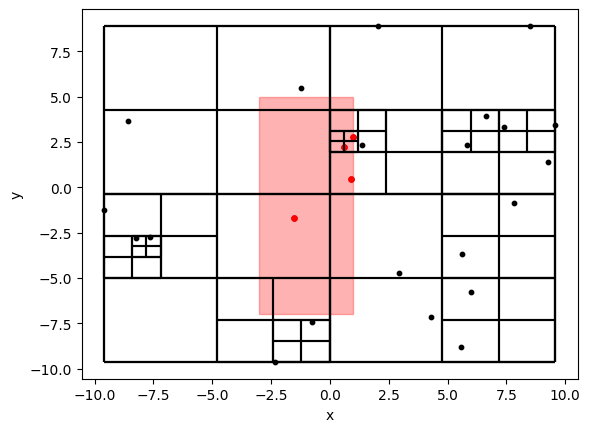
\includegraphics[width=0.7\textwidth]{images/quadtree_vis.png}
\end{figure}

Aby wygenerować plik GIF do wyświetlania kolejnych kroków algorytmu, należy zamiast:
\texttt{quadtree.vis.show()}, użyć \texttt{quadtree.vis.show\_gif()}.

\newpage

\subsection{Wizualizacja \texttt{KdTreeVis}}
Klasa \texttt{KdTreeVis} działa identycznie jak klasa \texttt{KdTree}, ale dodatkowo dodaje elemnty wizualizacji, zarówno podczas konstruowania drzewa jak i odpowiadania na zapytanie.

Przykładowe użycie klasy \texttt{KdTreeVis} dla losowo wygenerowanego zbioru punktów:

\begin{minted}{python}
    from kd_tree_visualization import KdTreeVis
    from geometry import Rectangle
    from numpy.random import seed, uniform

    seed(0)

    def generate_uniform_points(left, right, n):
        return list(zip(uniform(left, right, size=n), uniform(left, right, size=n)))
    

    points = generate_uniform_points(-10, 10, 25)
    rectangle = Rectangle(-3, 1, -7, 5)
    kd_tree = KdTreeVis(points)
    kd_tree.find(rectangle)
    kd_tree.vis.show()
\end{minted}

\begin{figure}[H]
    \centering
    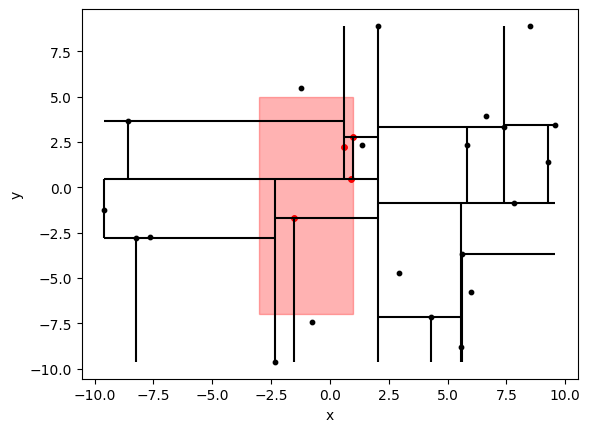
\includegraphics[width=0.7\textwidth]{images/kd_tree_vis}
\end{figure}

Aby wygenerować plik GIF do wyświetlania kolejnych kroków algorytmu, należy zamiast:
\texttt{kd\_tree.vis.show()}, użyć \texttt{kd\_tree.vis.show\_gif()}.

\section{Bibliografia}
\begin{enumerate}
    \item dr inż. Barbara Głut Wykład -- wyszukiwanie geometryczne.
\end{enumerate}

\end{document}